\documentclass[NETN,manuscript]{stjour-new}
\articletype{Research}
\usepackage{graphicx}
\usepackage{cleveref}
\graphicspath{ {figs/} }
% \documentclass{article} % This command is used to set the type of document you are working on such as an article, book, or presentation

\usepackage{geometry} % This package allows the editing of the page layout
\usepackage{amsmath}  % This package allows the use of a large range of mathematical formula, commands, and symbols
\usepackage{graphicx}  % This package allows the importing of images

\newcommand{\question}[2][]{
    \begin{flushleft}
    \textbf{Question #1}: \textit{#2}
    \end{flushleft}
}
\newcommand{\sol}{\textbf{Solution}:} %Use if you want a boldface solution line
\newcommand{\maketitletwo}[2][]{
    \begin{center}
        \Large{\textbf{Assignment #1}}

        Course Title

        \vspace{5pt}
        \normalsize{Matthew Frenkel}

        \today
        \vspace{15pt}
    \end{center}
}
% \documentclass{article}
% \usepackage[utf8]{inputenc}
% \usepackage{geometry}
% \usepackage{amsmath}
% \usepackage{graphicx}
% \usepackage[style=apa]{biblatex}
% \usepackage{natbib}
% \usepackage[font=footnotesize,labelfont=bf]{caption}
% \addbibresource{rmt.bib}
% \bibliographystyle{plain}
% \bibliography{rmt}
\begin{document}

\title{Random Matrix Theory Tools for the Analysis of Functional Magnetic Resonance Imaging Examinations}
\author[Derek M. Berger, Gurpreet S. Matharoo, Jacob Levman]{
    Derek M. Berger\affil{1},
    Gurpreet S. Matharoo\affil{2}
    \and Jacob Levman\affil{3}
}
\affiliation{1}{Computer Science, St. Francis Xavier University, Antigonish, Canada}
\affiliation{2}{Physics, St. Francis Xavier University, Antigonish, Canada}
\affiliation{3}{Computer Science, St. Francis Xavier University, Antigonish, Canada}

% \date{\today}

\keywords{random matrix theory, feature extraction, functional connectivity,
functional magnetic resonance imaging, voxelwise connectivity, predictive analysis}

\begin{abstract}
    Previous studies have investigated the potential of using analytic techniques from Random Matrix
    Theory (RMT) to investigate magnetic resonance imaging (MRI) data. We assess the potential
    application of RMT-based features for the analysis of functional MRI (fMRI) across diverse
    datasets. As novel contributions, we (1) assess the potential for RMT-inspired, whole-brain
    features extracted from voxel-wise functional connectivity to contain information useful for
    classifying between various psychological processes, (2) assess these features’
    predictive—rather than explanatory—value, (3) investigate the effect of varying RMT analysis
    methods on the robustness of study findings, and (4) make code publicly available to extract
    these features from a wide variety of data. We find preliminary evidence suggesting that
    RMT-inspired features may have unique potential in analyses of fMRI functional connectivity.
\end{abstract}

\section{Introduction}

In functional magnetic resonance imaging (fMRI), changes in the blood-oxygenation-level-dependent
(BOLD) signals are related to neural activity. It is common to investigate statistical relationships
between the BOLD signals through \textbf{functional connectivity} analyses, where correlations between
collections of these signals are examined to infer connections between different voxels or regions
of interest (ROIs) within the brain.

Whether in the presence of experimental stimuli, or the relative absence, as in a resting state,
complex functional connectivity networks are ubiquitous
\citep{bucknerBrainDefaultNetwork2008,foxCoverHumanBrain2005,gonzalez-castilloTaskbasedDynamicFunctional2018,hermundstadStructuralFoundationsRestingstate2013}.
This complexity suggests fMRI is a candidate to be studied using \textbf{Random Matrix Theory} (RMT), a set
of mathematical tools originally developed some 50 years ago to solve complex problems in nuclear
physics \citep{guhrRandommatrixTheoriesQuantum1998a,mehtaRandomMatrices2004}. In various
physical systems where nuclei can have different possible states, precisely modeling the entirety of
the interactions between nuclei is often intractable. For such large, complex systems, the
eigenvalues (or spectra) efficiently summarize the totality of the interactions between components
of the system, and RMT describes the expected behaviour of such eigenvalues. By analysing the
spectrum statistically, complex systems can be investigated by comparison to the universal
properties predicted by RMT.

\begin{sloppypar}
These universal properties have been observed in diverse phenomena. In small-scale systems, RMT
universalities have been observed in quantum chaotic systems, complex nuclei, atoms, molecules and
disordered mesoscopic systems
\citep{guhrRandommatrixTheoriesQuantum1998a,mehtaRandomMatrices2004,brodyRandommatrixPhysicsSpectrum1981,beenakkerRandommatrixTheoryQuantum1997,bohigasHigherOrderCorrelationsSpectra1985,wintgenLevelStatisticsQuantized1988,pandeySkewOrthogonalPolynomialsUniversality2001},
and at larger scales, RMT has been applied to atmospheric physics
\citep{santhanamStatisticsAtmosphericCorrelations2001}, stock cross-correlations
\citep{plerouRandomMatrixApproach2002} , social networks
\citep{jalanUncoveringRandomnessSuccess2014}, random networks
\citep{bandyopadhyayUniversalityComplexNetworks2007}, network-formation in liquids
\citep{sastrySpectralStatisticsInstantaneous2001,matharooSpectralStatisticsQuenched2009}  and
amorphous clusters
\citep{sarkarUniversalityVibrationalSpectra2004,matharooVibrationalSpectraAmorphous2005,matharooUniversalityVibrationalSpectra2008}.
Within biological systems, RMT has also been used to successfully model aspects of  amino acid
functional relationships \citep{bhadolaTargetingFunctionalMotifs2016}, synchrony in epileptic
seizures \citep{osorioPhasesynchronizationRandommatrixBased2011}, and in protein-protein
interactions both in different species \citep{agrawalQuantifyingRandomnessProtein2014} and breast
cancer \citep{raiRandomnessPreservedPatterns2015}.
\end{sloppypar}

In recent years, RMT analyses have been applied to study brain functioning.  The earliest  study
demonstrated that spectra of the correlations between electroencephalographic (EEG) signals closely
resemble those of the Gaussian Orthogonal Ensemble (GOE) \citep{sebaRandomMatrixAnalysis2003}.
Somewhat more recently, RMT was used to evaluate the quality of whole brain features extracted from
fMRI data \citep{voultsidouFeatureEvaluationFMRI2007,verganiRestingStateFMRI2019}. RMT has also
been used in diffusion MRI to aid in the selection of the number of components to employ in
principal-component reduction analysis and denoising
\citep{veraartDenoisingDiffusionMRI2016,verganiRestingStateFMRI2019,ulfarssonDimensionEstimationNoisy2008}.

Finally, RMT has been used in ROI-based fMRI functional-connectivity studies to investigate
differences between rest and task states \citep{wangSpectralPropertiesTemporal2015}, between
subjects with and without ADHD \citep{wangRandomMatrixTheory2016}, and between pain and non-pain
states \citep{matharooSpontaneousBackpainAlters2020}. Across these three studies, the spectra of
resting or low-attention states exhibited properties closest to the GOE. These findings suggest that
certain aspects of psychological processes might be characterized, in part, by features computed
from the eigenvalues of fMRI correlation matrices, and that these features might vary in an
interpretable manner across psychological processes. If this is the case, RMT could have unique
potential in characterizing the functioning of the human brain.

Here, we use a novel, voxel-based approach, and expand the applications of RMT to analyze fMRI scans
from  diverse datasets. We extract RMT-inspired whole-brain features from \textbf{voxelwise
functional connectivity} data, and assess the predictive value of these features. We also examine in
detail the robustness of the RMT methodology to various common analytic choices.

\section{Materials and Methods}

\subsection{Datasets}

As our primary intention is to examine the potential utility of RMT-derived features across a wide
variety of data, and not to decisively put forward or refute any specific hypotheses relating RMT to
psychological processes, we examine a wide selection of fMRI datasets available on the
\href{https://openneuro.org/}{OpenNeuro} platform [36].  This allows for a broad assessment of the
potential of voxelwise RMT features.

However, since previous studies employing RMT for feature extraction have partially interpreted
their findings with respect to attentional processes
\citep{wangRandomMatrixTheory2016,matharooSpontaneousBackpainAlters2020}, we have elected to use
datasets that involve attention in some way. This includes measures of attention or vigilance, or
comparisons between a condition involving more attention and focus (e.g. a task state) or conditions
which should involve considerably less attention or focus (e.g. resting-state).

Dataset scan parameters and acquisition details are summarized in Table \ref{table:1}, and sample
and subgroup sizes are summarized in Table \ref{table:2}. For all datasets, we use the raw
(unpreprocessed) scans, and perform our own preprocessing (detailed later). Given the complexity of
these datasets, we highlight below only those aspects relevant to the current paper.

\begin{table}[h!]
\small
\centering
\begin{tabular}{ c c c c c c c }
\hline
\textbf{ID}  & \textbf{FOV (mm)}  & \textbf{Dimensions}  & \textbf{Voxel size (mm)} & \textbf{TR} & \textbf{Volumes} & \textbf{Time (s)} \\
\hline
PSYCH   &  192              & 128 x 128 x 70 & 1.5 x 1.5 x 1.5 & 3.0 & 300 & 15 \\
OSTEO   &  -                & 64 x 64 x 36   & 3.4 x 3.4 x 3.0 & 2.5 & 300 & 12.5 \\
REFLECT &  210              & 72 x 72 x 46   & 3.0 x 3.0 x 3.0 & 2.5 & 204 & 10.2 \\
REFLECT &  240              & 64 x 64 x 33   & 3.8 x 3.8 x 3.8 & 2.0 & 260 & 8.7 \\
PARK    &  240 x 240 x 129  & 80 x 80 x 43   & 3.0 x 3.0 x 3.0 & 2.4 & 149 & 5.96 \\
LEARN   &  -                & 64 x 64 x 36   & 3.0 x 3.0 x 3.0 & 2.0 & 196 & 6.5 \\
\hline
\end{tabular}
\caption{
    ID = Identifier for paper. FOV = Field of View. TR = Time of Repetition (seconds).
    Time = total duration (minutes) of each scan. Dimensions listed as M x N x P,
    indicate P slices with dimensions M x N.
}
\label{table:1}
\end{table}


\begin{table}[h!]
\small
\centering
\begin{tabular}{ l l c c c }
\hline
\textbf{ID}  & \textbf{Subgroup / Condition}  & \textbf{Subjects}  & \textbf{Task} & \textbf{Scans per Subject} \\
\hline
PSYCH   &  high\_vigilance    & 12 / 11 & resting-state                    & 2 \\
        &  low\_vigilance     & 10 / 11 & resting-state                    & 2 \\
        &  trait\_attend      & 12 / 15 & resting-state                    & 2 \\
        &  trait\_non-attend  & 10 / 7  & resting-state                    & 2 \\
        &  task\_attend       & 13 / 15 & resting-state                    & 2 \\
        &  task\_nonattend    &  9 / 7  & resting-state                    & 2 \\
\hline
LEARN   &  task              & 24      & learn image sketches & 16 \\
        &  rest              & 24      & resting-state                    & 2 \\
\hline
REFLECT &  control (no pain) & 20      & resting-state                    & 1 \\
        &  duloxetine        & 19      & resting-state                    & 1 \\
        &  placebo           & 37      & resting-state                    & 1 \\
        &  allpain (duloxetine + placebo) & 56         & resting-state    & 1 \\
\hline
PARK    &  Parkinson's       & 17      & ANT                              & 6 \\
        &  control           & 17      & ANT                              & 6 \\
\hline
ECHO    &  summed/interleave & 31      & resting-state                    & 1 \\
        &  summed/interleave & 31      & imagery/reflection               & 4 \\
\hline
\end{tabular}
\caption{
    ID = Identifier for paper. FOV = Field of View. TR = Time of Repetition (seconds).
    Time = total duration (minutes) of each scan. Dimensions listed as M x N x P,
    indicate P slices with dimensions M x N.
}
\label{table:2}
\end{table}


\subsubsection{Dataset 1}
Dataset 1 (referred to in figures and tables with the label ``PSYCH'') has detailed and extensive
information available in \cite{gorgolewskiHighResolution7Tesla2015}. Subjects completed a battery of
psychological measurements, and various resting-state fMRI (rs-fMRI) images were obtained. Only the
whole-brain 7-Tesla rs-fMRI scans were used for the current paper, to make the results comparable to
the other included datasets. For the purpose of keeping with the ``attention'' theme of the analyses
in this paper, three pairings of subgroups were constructed via z-score splits of the various
sum-scores of scale items involving concepts closely related to attention.

\emph{Trait Attention}.
The PANAS-X \citep{watsonPANASXManualPositive1994} is a 9-point Likert-type self-report measure
that queries the extent to which subjects agree particular affective terms have applied to them over
a recent time period (e.g. a few weeks). An ad hoc (i.e. face-valid) sum-score was constructed from
the scale items: ``attentive'', ``alert'', ``interested'', ``concentrating'', and reverse-scored items
``sluggish'', ``tired'', ``sleepy'', ``drowsy''. Subjects with a z-score greater / less than zero on this
sum-score were placed in the high / low ``trait attention'' category

\emph{Task Attention}.
The Conjunctive Continuous Performance Task (CCPT;
\cite{shalevConjunctiveContinuousPerformance2011} is a behavioural measure of sustained attention
where subjects must react only if they see a red square among other different coloured figures. For
this paper, a sum score was constructed by subtracting the number of false positive and false
negative responses from the number of success responses, and subjects with a z-score greater / less
than zero on this scale were placed in high / low ``task attention'' category.

\emph{Vigilance}.
The Mini New York cognition questionnaire assesses various elements of the subject's cognitive
state, e.g. ``my thoughts involved other people'', ``I thought about something positive'' (translated
from German; \cite{gorgolewskiCorrespondenceIndividualDifferences2014}. One question assesses
alertness (``I was fully awake'' / ``war ich vollkommen wach'') and was used to create high / low
``vigilance'' conditions in the same manner as the previous two splits.

\subsubsection{Dataset 2}
Dataset 2 (referred to in figures and tables with the label ``OSTEO'') is detailed in
\cite{tetreaultBrainConnectivityPredicts2016}. Subjects included healthy controls (``nopain''
condition) and individuals with knee osteoarthritis (``pain'' condition) treated for 2 weeks with
either placebo (``pain'' condition) or duloxetine (``duloxetine'' condition). An additional grouping was
also created with both the placebo and duloxetine data (``allpain'' condition), allowing for six
subgroup comparisons. All subjects were imaged with whole-brain rs-fMRI. Scan parameters are
documented in Table \ref{table:1}. The use of rs-fMRI and RMT for examining pain makes this dataset
complementary to \cite{matharooSpontaneousBackpainAlters2020}.

\subsubsection{Dataset 3}
Dataset 3  (referred to here with the label ``REFLECT'', due to the ``reflective” nature of the
cognitive tasks) is described in full detail by \cite{dupreMultiechoFMRIReplication2016}. Both
multi-echo rs- and task-fMRI scans were conducted with scan parameters summarized in Table \ref{table:2}. Tasks
involved viewing various affective images \citep[see][for details]{sprengPatternsBrainActivity2010}
and performing tasks related to autobiographical memory, prospection, or theory-of-mind reasoning.
Continuing with the theme of broadly comparing high versus low attention throughout this paper, the
different tasks were simply treated generically as ``attending'', in contrast to the non-attentive
resting-state scans. This resulted in four task state scans and one resting-state scan per subject.

In order to combine the multi-echo data into a single, usable matrix, two methods were employed. In
the ``summed'' condition, echoes were combined via summation, a method which has value in providing an
image with overall increased contrast \citep{kunduMultiechoFMRIReview2017}. In the ``interleave''
condition, echoes were interleaved at each voxel: that is, if we denote the voxel's \(i\)th signal value
from echo \(j\) as \(t_{j,i}\), then the interleaved voxel of the new image has the time-series \([t_{1,1},
t_{2,1}, t_{3,1}, \dots, t_{1,i}, t_{2,i}, t_{3,i}, \dots, t_{1,n}, t_{2,n}, t_{3,n}]\).

This creates a physically-meaningful 4D image that contains the full, original multi-echo fMRI
time-series data without any alterations. It should be noted that the purpose of these combination
methods is not to create a 4D volume that allows optimal detection of the purely task-linked BOLD
signal, but to ensure all scan information was used with minimal additional analytic assumptions.

\subsubsection{Dataset 4}
Dataset 4 (referred to in figures and tables with the label ``PARK'' or ``PARKINSONS'') is documented and
described in detail in \cite{madhyasthaDynamicConnectivityRest2015}. Scan parameters are documented
in Table \ref{table:1}. Subjects with non-demented Parkinson’s Disease (PD) and healthy controls performed a
number of repetitions of the Attention Network Task
\citep[ANT;][]{fanActivationAttentionalNetworks2005}. Subgroup details are available in Table \ref{table:1}. As the ANT
task demands high attention, it is not as straightforward to create ``high'' or ``low'' attention
groups. Instead, since attention presumably is high and varies little in this dataset, and subgroups
instead differ by virtue of the presence or absence of PD, any results here serve as a useful
comparison point for the results from studies that should clearly involve attentional differences.
This dataset also included extensively preprocessed scans, which were included in analyses to
examine the effects of preprocessing on the extracted RMT features.

\subsubsection{Dataset 5}
Dataset 5 (referred to in figures and tables with the label ``LEARN'') is documented and described in
detail in \cite{schapiroHumanHippocampalReplay2018}. In this study, both rs-fMRI and task fMRI scans
were available for all subjects, allowing for within-subject comparisons. The complex task involved
multiple phases, wherein subjects were exposed to named, black-and-white outlined satellite images
related by family-resemblance of the components \citep[see figure 1
of][]{schapiroHumanHippocampalReplay2018}. After this learning task, subjects were tested on their
memory of the various learned features. Scans corresponding to both the initial learning and
subsequent testing phase were included in the high-attention ``task'' subgroup for the purposes of
the analysis of this paper. Resting state scans were included in the low-attention ``rest''
subgroup.

\subsection{Preprocessing}
Some consideration should be given to whether it is appropriate to apply standard preprocessing
steps before extracting RMT features, as preprocessing steps should be developed, tested, and
employed always with respect to a set of inferential goals and a specific analytic framework.
However, these preprocessing steps are increasingly recognized to have complex effects on fMRI
analyses \citep{parkerBenefitSliceTiming2019}. For example, spatial smoothing has clear benefits
when employing a general linear model
\citep{miklEffectsSpatialSmoothing2008,alakorkkoEffectsSpatialSmoothing2017,worsleyAnalysisFMRITimeSeries1995},
but is less motivated in functional network analyses with small ROIs, where the effect of smoothing
can be considerable
\citep{alakorkkoEffectsSpatialSmoothing2017,goelmanMaximizingNegativeCorrelations2014,trianaEffectsSpatialSmoothing2020},
with these effects interacting complexly with factors like field strength and image resolution
\citep{triantafyllouEffectSpatialSmoothing2006}. Similarly, image registration is usually required
to allow comparisons across (or even within) subjects, but the choice of registration strategy can
have dramatic effects on functional network analyses \citep{magalhaesImpactNormalizationSegmentation2014}.

The RMT features extracted here are based on functional correlations rather than ROI activations,
and are completely insensitive to voxel location (spatial re-arrangement of an image’s voxels does
not change the eigenvalues of the correlation matrix). Thus RMT features summarize all voxel-wise
correlations in a whole-brain and location-free manner, which brings into question some of the usual
motivations for performing spatial smoothing, or registration to identify ROIs. In addition, if
image dimensions are identical between subjects, the RMT features (by virtue of their definition and
the \textbf{unfolding} procedure) already allow for direct comparisons. Thus, the usual motivations for
registration are also no longer clear when extracting RMT features.

Given these particularities, as well as the novelty of the RMT-based methods and the diversity of
the datasets, we elected to minimize the complexity of the preprocessing pipeline to ensure that
data processing is kept as standardized as possible. Ultimately, different preprocessing pipelines
for RMT fMRI analyses can be expected to have different benefits and shortcomings depending on the
question being investigated, and possibly also the specific RMT features being relied upon, but such
an investigation is beyond the scope of the current study.

For this paper’s analyses, brain extraction is necessary to limit analyses to the appropriate
voxels, motion correction is necessary to allow proper brain extraction, and both motion-correction
and slice-time correction simplify the interpretation of voxel-voxel correlations across voxel
locations. Whereas physiological noise regression and bias field correction would perhaps be
appropriate here, there is insufficient data to perform these steps for all datasets (Table \ref{table:2}).
Thus, motion-correction was performed with FSL's MCFLIRT
\citep{jenkinsonImprovedOptimizationRobust2002}, slicetime correction with the default method in
FSL, and brain extraction was performed with BET \citep{smithFastRobustAutomated2002}. Due to
differences in the size of the REFLECT data, the higher-resolution resting-state data was
interpolated to have the same spatial dimensions as the task data.

\subsection{RMT-Derived Features}
This paper examines features informed by various aspects of RMT, and which can be extracted from
empirical correlation matrices. To keep with previous studies, we limit our analyses to features
extracted only from the eigenvalues of the matrices of correlations between all voxel signals.

Two classes of features were examined in this study: those that require unfolding, and those that do
not. In order to compare the observed eigenvalue distribution to some theoretical predictions, the
eigenvalues must be unfolded \citep{guhrRandommatrixTheoriesQuantum1998a,mehtaRandomMatrices2004}.
The details and motivation behind the unfolding procedure are well documented in
\cite{guhrRandommatrixTheoriesQuantum1998a}. Practically, the unfolding process can be viewed as a
smoothing and rescaling procedure where the originally observed spectrum \(\lambda_1 \le \dots \le
\lambda_n\) is smoothly mapped to the unfolded spectrum \(e_1, \dots, e_n\), such that \(\sum d_i/n
\approx 1\), if \(d_i = e_{i+1} - e_i \). For most empirical data, the true smoothing function is
not known, and so must be approximated
\citep{guhrRandommatrixTheoriesQuantum1998a,mehtaRandomMatrices2004}. Typically, a polynomial is
chosen \citep{abul-magdUnfoldingSpectrumChaotic2014}.

A number of statistics or ``spectral observables'' \citep{mehtaRandomMatrices2004} can then be
computed from this unfolded spectrum. In the literature, the two most common points of comparison
for these unfolded features are typically the features of the Poisson or Gaussian Diagonal Ensemble
(GDE) and the GOE
\cite[see e.g.][]{santhanamStatisticsAtmosphericCorrelations2001,jalanUncoveringRandomnessSuccess2014,bandyopadhyayUniversalityComplexNetworks2007,agrawalQuantifyingRandomnessProtein2014,raiRandomnessPreservedPatterns2015,
sebaRandomMatrixAnalysis2003,wangSpectralPropertiesTemporal2015,wangRandomMatrixTheory2016}. The
GOE (or GDE) consists of real, symmetric matrices where entries (or only diagonal entries) are
normal random variables with zero mean and unit variance. When the empirically observed features are
close to those of the GOE, this is usually interpreted as indicating a high degree of randomness and
statistical independence in the data, and when the observed features are closer to those expected in
the GDE or Poisson case, this is interpreted as indicating a high degree of coherence or dependence
\citep{santhanamStatisticsAtmosphericCorrelations2001,jalanUncoveringRandomnessSuccess2014,bandyopadhyayUniversalityComplexNetworks2007,agrawalQuantifyingRandomnessProtein2014,raiRandomnessPreservedPatterns2015,
sebaRandomMatrixAnalysis2003,wangSpectralPropertiesTemporal2015,wangRandomMatrixTheory2016,matharooSpontaneousBackpainAlters2020}.

The Nearest-Neighbours Spacings Distribution (NNSD) is the most basic RMT feature, and is the
distribution of the spacings (differences) of adjacent unfolded eigenvalues. Normally, the NNSD is
analysed visually via a histogram of the distribution of spacings, however it is also possible to
analyse it more formally by fitting the Brody distribution \citep{brodyStatisticalMeasureRepulsion1973}:

\[
p(s) = \alpha (1 + \beta) s^\alpha \exp({\beta s^{\alpha+1}}),
\quad \alpha = \left[ \Gamma \left( \frac{\beta+2}{\beta+1} \right) \right]^{\beta+1}
\]

where \(\beta\) is free to vary within \([0, 1]\), with \(\beta = 0\)  producing the expected NNSD
for the GDE case, and \(\beta = 1\) producing the expected NNSD for the GOE case. In this paper, we
fit, via maximum likelihood, the empirically observed spacings with the Brody distribution, and
report the Brody parameter, \(\beta\), as an important unfolded feature to investigate.

Whereas the NNSD and Brody parameter characterize the local properties of eigenvalues close on the
spectrum, the long-range properties relating eigenvalues distant on the spectrum can be
characterized by both the spectral rigidity and level number variance
\citep{guhrRandommatrixTheoriesQuantum1998a,mehtaRandomMatrices2004}. The spectral rigidity,
\(\Delta_3(L)\), is calculated for any real value \(L\) as:

\[
\Delta_3(L) = \left \langle \min_{A,B} \frac{1}{L} \int_c^{c+L} \left(  \eta(\lambda) -A \lambda - B \right)^2 \right \rangle_c
\]

where \(\eta(\lambda)\) is the number of unfolded eigenvalues less than or equal to \(\lambda\),
\(\langle \cdot \rangle_c\) denotes the average with respect to all starting points \(c\), and where
\(A\) and \(B\) denote the slope and intercept, respectively, of the least squares fit of a straight
line to \(\eta(\lambda)\) on \([c, c+L]\) \citep{guhrRandommatrixTheoriesQuantum1998a}. The level
number variance, \(\Sigma^2(L)\), is closely related to the spectral rigidity
\citep{mehtaRandomMatrices2004}, and is calculated as:

\[
\Sigma^2(L) = \left\langle \eta^2(L, c) \right\rangle_c - \left\langle \eta(L, c) \right\rangle^2_c
\]

where \(\eta(L, c)\) is the number of unfolded eigenvalues in \([c, c+ L]\), and where \(c\), \(L\),
and \(\langle \cdot \rangle_c\) are as above \citep{guhrRandommatrixTheoriesQuantum1998a}. Both the
spectral rigidity and level number variance are also computed and investigated in this study.

In addition to the unfolded features suggested by RMT, there are some potential ``raw'' features that
do not require an unfolding procedure. The entire eigenvalue spectrum likely contains important
information related to the system, and is also investigated as an RMT-inspired feature.

The distribution of eigenvalues of large rectangular matrices with finite-variance, independent and
identically distributed (\textit{i.i.d.}) entries also converges to the Marchenko-Pastur (MP)
distribution \citep{marcenkoDISTRIBUTIONEIGENVALUESSETS1967,yaoLargeSampleCovariance2015}:

\[
\rho(\lambda) =
\frac{1}{2\pi\sigma^2}
\frac{\sqrt{(\lambda_+ - \lambda)(\lambda - \lambda_-)}}{r\lambda}, \;
\lambda_{\pm} = \sigma^2\left(1 \pm \sqrt{\lambda}\right)^2
\]

where \(\sigma^2\) is the true variance of the distribution of each i.i.d. entry (equal to 1 in the
case of correlation matrices), and where \(r = N / T\), for matrices of dimension \(N \times T\).
While real-world data will not, in general, be i.i.d., the extent to which spectra overlap with or
are well-described by the MP distribution has been used to guide analytical decisions regarding the
relevance of empirically observed eigenvalues. That is, since the majority of the eigenvalues of
random correlation matrices will fall within \([\lambda_{-}, \lambda_{+}]\), eigenvalues observed to
fall within this region are typically considered to be the result of noise
\citep{veraartDenoisingDiffusionMRI2016,veraartDiffusionMRINoise2016,ulfarssonDimensionEstimationNoisy2008,macmahonCommunityDetectionCorrelation2015}.
We examine as a potential feature the proportion of eigenvalues that fall within this range, and
call this the \textbf{noise ratio}. In addition, we calculate a broader, shifted noise ratio, based on the
adjustments of \cite{almogUncoveringFunctionalSignature2019} which takes into account the larger
degree of correlation in empirical data.

\subsection{RMT Feature Extraction}
The entire 4-dimensional \(m \times n \times n \times p \times t\) scan array for each run,
excluding voxels with constant signals (which lead to undefined correlations), and excluding voxels
identified as non-brain via preprocessing, was flattened to a two-dimensional \(m \cdot n \cdot p
\times t\) matrix, and then the \(t - 1\) eigenvalues of that correlation matrix were computed. The
value of \(t\) for a scan can be inferred from the number of volumes in Table \ref{table:1}. The
various RMT features mentioned above were then extracted via the \texttt{empyricalRMT} library
\citep{bergerStfxecutablesEmpyricalRMTPreliminary2020} developed and made publicly available as part
of this study, as well as via code for this paper \citep{bergerderekm.DMBergerRandommatrixfmriV02020}.

As both the spectral rigidity and level number variance can be highly sensitive to the choice of
smoothing procedure used in the unfolding method
\citep{abul-magdUnfoldingSpectrumChaotic2014,moralesImprovedUnfoldingDetrending2011,abueleninSpectralUnfoldingChaotic2018,fossionRandommatrixSpectraTime2013,abueleninEffectUnfoldingSpectral2012},
all unfolded features in this study were calculated using polynomials of degree 5, 7, 9, 11, and 13
as the smoothing technique. As much of the variance in the unfolded spectral statistics can be due
to the largest eigenvalues acting as anchor points during smoothing
\citep{moralesImprovedUnfoldingDetrending2011,abueleninEffectUnfoldingSpectral2012}, all unfolded
features were also calculated twice (in addition to each polynomial degree) to examine the effects
of trimming on spectral observables: once with only the largest eigenvalue omitted, and once with
the largest 20 eigenvalues omitted.

\subsection{Feature Evaluation}
To evaluate the extracted RMT features, for each possible pairing of subgroups in each dataset, each
feature was used to predict subject subgroup membership. That is, for each dataset, and for each
possible pairing of subgroups, all scans belonging to a subgroup were pooled together and treated as
independent samples of the subgroup of interest. So, for example, in the LEARN dataset, this
resulted in a comparison of 384 (\(16 \times 4\)) task scans, to 48 (\(2 \times 24\)) rest scans. When it was not
reasonable to compare scans across sessions, sessions were analyzed separately. This was the case
for the PSYCH dataset, where psychological measurements, and thus subgroups, differed from session
to session.

A wide variety of standard, out-of-the-box classifiers available in the Python scikit-learn library
\citep{pedregosaScikitlearnMachineLearning2011} were then employed to gauge the predictive value of
the RMT features. To allow for a wide range of flexibilities, classifiers employing k-nearest
neighbours (KNN), with k values in \(\{1, 2, 3, \dots, 10, 20\}\), logistic regression (LR), linear
discriminant analysis (LDA), and a support-vector machine (SVM) were employed. Default parameter
values were used when possible \citep[see][for precise function calls used]{bergerderekm.DMBergerRandommatrixfmriV02020}.

The accuracy of each binary classifier was then validated with leave-one-out cross-validation
(LOOCV) on all datasets, for all combinations of trimming and unfolding choices.

\section{Results}

\subsection{Overview}
Due to space limitations, we highlight only key results here. Extensive overviews of the full
results are available in the supplementary materials. Visual summaries of the prediction accuracies
for all features and analytic choices are presented in figures S1--4. Prediction accuracies for only the
multivariate RMT features are summarized in figures S5--7, and the distributions of the scalar features
are presented in figures S8--10. Prediction accuracies for the scalar features across analytic choices
are summarized in figures S11--12.

Numeric (mean) summaries across datasets, broken down by classifier and feature are available in
Tables S11--18. Complete (unsummarized) tables of all predictions for all combinations of features,
unfolding degree, and trimming are available as supplementary material in the spreadsheet
\texttt{prediction\_tables\_fullpre.ods}. Unless otherwise noted, subsequent figures and analyses were
computed using the preprocessed data: full results for the raw data are available as spreadsheets in
the supplementary material in \texttt{prediction\_tables.ods}.

With the exception of the LEARNING dataset, the RMT-inspired features all demonstrated some
predictive utility (figures S1-4). For example, there were strong differences in RMT features between
task and rest conditions for the REFLECT dataset, but the features were of variable predictive
utility in the PSYCH dataset, sometimes outperforming the naïve classifier, and sometimes not.
Although the RMT features were useful in the comparison involving duloxetine and controls (no pain)
in the OSTEO dataset, these features mostly did not aid in classifying between any of the other
possible pairings of subgroups in this dataset (figures S1-4).

Although the performance of classifiers trained on RMT features was variable, there was a tendency
for the raw and largest eigenvalues to be the most predictively useful features, especially in the
REFLECT and PARK data in discriminating between Parkinson's and controls (figures S5-7. S13; but see
Discussion).

\subsection{Raw Features}
As evident from figures S8-10, the scalar raw features (largest eigenvalue, noise ratio, and shifted
noise ratio) varied more within than between subgroups. They were not generally useful for
classifying conditions (Tables S15-17), with two or three notable exceptions.

The noise ratio (but not shifted noise ratio) differed consistently between the duloxetine and
control groups in the OSTEO data, allowing for prediction accuracies of up to 72\% compared to 51\%
for the naive classifier (figures S11-12 top-right panel, Table S5). The largest eigenvalue was also
useful in distinguishing between subjects self-reporting high versus low vigilance across sessions:
accuracies up to 64\% and 65\% (compared to naïve accuracies of 55\% and 50\%) for the first and
second sessions, respectively (Table S6). Finally, for the REFLECT data, task and rest were
perfectly distinguishable with various features and with some classifiers.

The sorted, raw eigenvalues, however, more consistently contained information that allowed some
separation of subgroups. Averaging across all datasets and comparisons, the raw eigenvalues
consistently demonstrated predictive utility (Tables S7--8). As visible in figures S13, the eigenvalues
had the most consistent predictive value for distinguishing individuals with Parkinson's from
controls, or distinguishing those with osteopathic pain taking duloxetine from controls (``nopain'' in
Fig. S13). The raw eigenvalues sometimes had predictive value for the PSYCH data, most notably in
comparing those differing in self-reported vigilance and high vs. low scorers in the attention task
(Table S7--8).

In all these relationships, normalizing the eigenvalues to the interval \([0,1]\) prior to
prediction considerably improved prediction accuracy (Tables S9-12).

\subsubsection{Role of Classifer}
The raw eigenvalues generally had the most predictive utility when employing either an SVM
classifier or KNN classifier with \(k > 3\) (Table S11, first row). When the raw eigenvalues were
first min-max normalized prior to prediction, an SVM classifier was clearly the most consistent in
predicting subgroup memberships (Table S12), however without normalization, KNN with \(k = 8\) or
\(k = 9\) generally best predicted subgroup membership across datasets (Table S11).

\subsection{Unfolded Features}
The Brody parameter rarely resulted in predictions exceeding naïve accuracies in these comparisons:
for most unfoldings and comparisons, the Brody parameter was either constant and equal for all
subjects (e.g. exactly 0.999 or 0.0001) or deviated from these values only for a small number of
subjects. This is because the observed NNSDs were usually well outside of the GOE-GDE bounds.

The predictive utility of the unfolded RMT features varied considerably across datasets and
classifiers. However, some results were robust: for example, the spectral rigidity and level number
variance strongly differentiated controls from individuals prescribed duloxetine for osteopathic
pain, and this differentiation persisted regardless of unfolding degree or trimming
(\cref{fig:levelvar,fig:nnsd,fig:rigidity}, top-right panels).

Despite the insensitivity to unfolding in this dataset, there was still nontrivial variability in
accuracy across classifiers when classifying duloxetine vs controls, with the less flexible
classifiers (logistic regression, SVM, and KNN with k=10, 20) generally performing best (Tables
S1-2).

For other datasets, the predictive utility of the unfolded features was highly dependent on the
unfolding degree, and sometimes trim proportions. These differences are illustrated in detail for
the Parkinson's data in figures S14. For example, with minimal trimming, subgroup overlap in spectral
rigidity was minimized for unfolding degrees 5 and 9 (Fig. S14, first row), but with greater
trimming, this was not the case (Fig. S14, second row). For the level number variance with minimal
trimming, subgroup overlap appeared smaller for lower unfolding degrees (Fig. S14, third row),
however, with a greater degree of trimming, separation was clearer for slightly larger degrees (Fig.
S14, fourth row).

Across datasets, the unfolding degree, compared to trimming, was a much more significant source of
variance in the overall predictive utility of the unfolded features (e.g. note the minimal changes
from trimming in Fig. S5 and S6, compared to the overall differences in prediction patterns from
differing choices of unfolding degree in Fig. S3 and S4). However, neither the choice of unfolding
degree nor amount of trimming had any easily summarizable effects on the predictive value of the
various RMT metrics: the optimal trimming and unfolding degree was different for each dataset and
comparison.

\subsubsection{Role of Classifier}. Across all datasets, unfoldings, and trimmings, the spectral rigidity was
generally best able to separate between subgroups when either k was large (10 or 20) in KNN, or
Logistic Regression or SVM was employed (Table S13). The pattern was similar for the level number
variance, although the predictive utility of the level number variance was, overall, slightly more
variable than the spectral rigidity (Table S4).

\section{Discussion}
In this study, certain features inspired by RMT and derived from the sorted eigenvalues of the full,
whole-brain voxelwise correlation matrix were found to contain information with the potential to
meaningfully differentiate between different neuropsychological phenomena. In addition to evidence
from previous studies
\citep{sebaRandomMatrixAnalysis2003,wangRandomMatrixTheory2016,matharooSpontaneousBackpainAlters2020}
this suggests RMT may be a useful analytic and theoretical tool for understanding functional
connectivity.

Although the choice of unfolding and trimming often had nontrivial effects on the overall shape and
values of the various spectral observables, and thus the predictive utility, in cases where there
was clear predictive utility, there was some evidence that the unfolding and trimming procedures did
not reverse the relations between subgroups (Fig. 1-3, S14). For example, regardless of the
unfolding methodology, it was always the case that control subjects had spectral observables
farthest from those of the GOE (Fig. 1-3) compared to those given duloxetine for osteopathic pain,
whereas when comparing subject's with Parkinson's to controls, Parkinson's subjects consistently
showed the greatest deviation from the GOE (Fig. S14).

\begin{figure}[ht]
\centerline{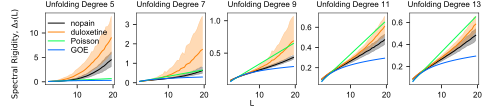
\includegraphics[width=\textwidth]{figure1}} \caption{
    (Colour online) Spectral rigidity for controls (nopain) vs. those with osteopathic pain taking
    duloxetine, trimming largest eigenvalue only. Solid lines indicate group mean rigidity, and
    shaded regions correspond to 99\% percentile bootstrapped intervals for each group. Vertical
    axes vary to better depict group-wise overlap.}
\label{fig:rigidity}
\end{figure}

\begin{figure}[ht]
\centerline{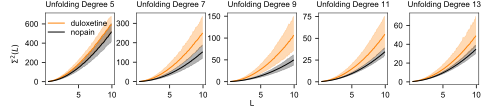
\includegraphics[width=\textwidth]{figure2}} \caption{
    (Colour online) Level variance for controls (nopain) vs. those with osteopathic pain taking
    duloxetine. Solid lines indicate group mean level variance, and shaded regions correspond to
    99\% percentile bootstrapped intervals for each group.  Vertical axes vary to better depict
    group-wise overlap.
}
\label{fig:levelvar}
\end{figure}

\begin{figure}[ht]
\centerline{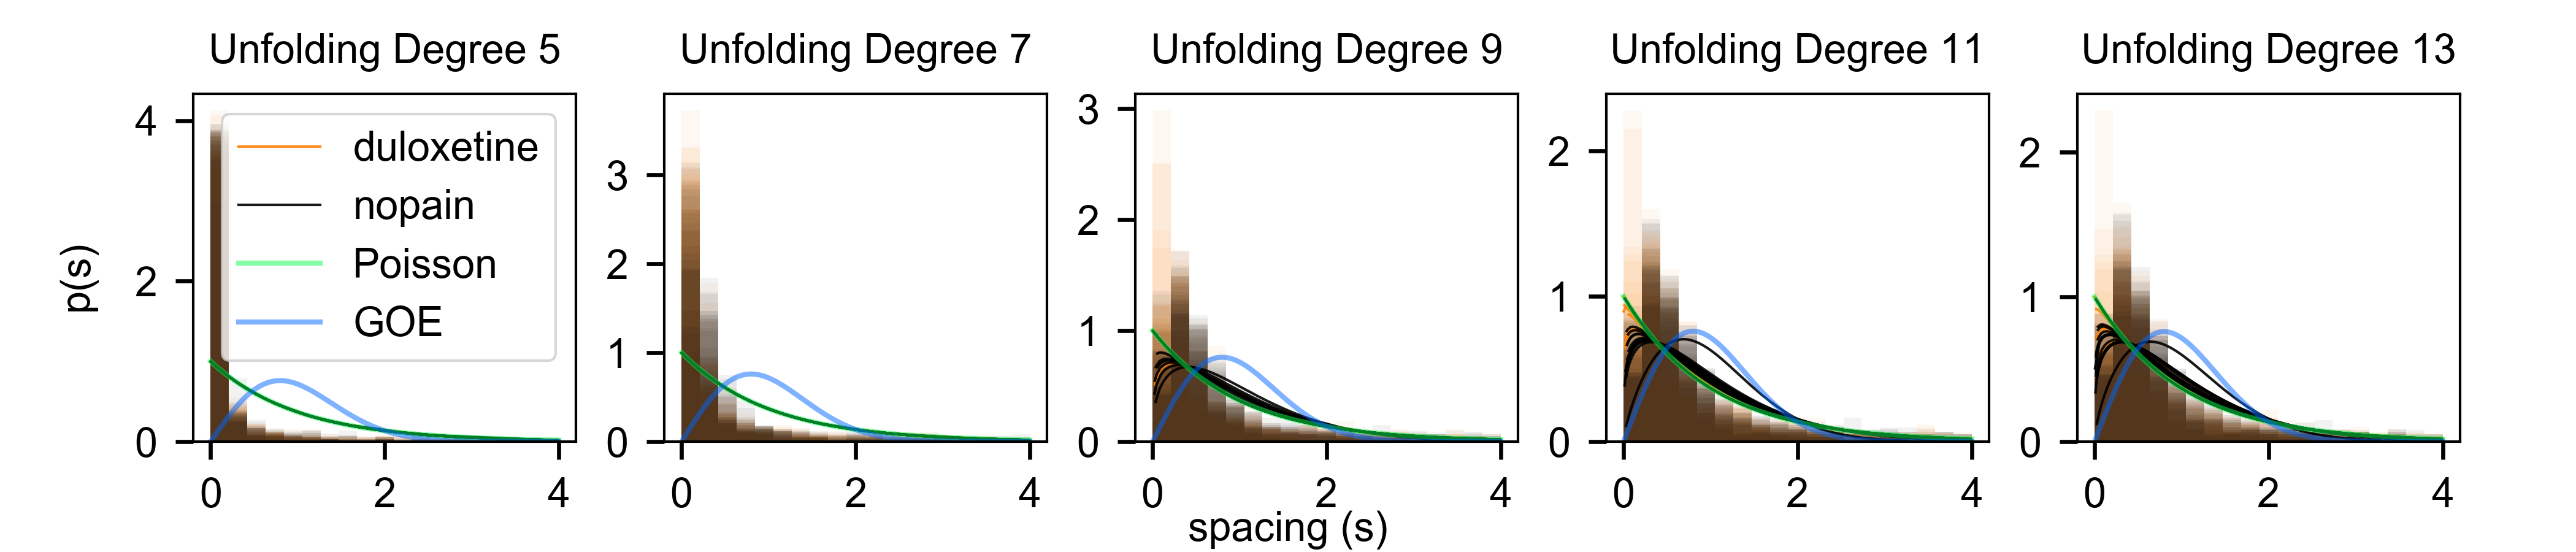
\includegraphics[width=\textwidth]{figure3}} \caption{
    (Colour online) Nearest Neighbours Spacings Distribution for controls (nopain) vs. those with
    osteopathic pain taking duloxetine. Solid lines indicate Brody distribution maximum likelihood
    estimates, and transparent regions depict the overlapping spacings histograms for all subjects.
}
\label{fig:nnsd}
\end{figure}


In particular, for some psychological phenomena examined in this study (specifically, the
resting-state, voxelwise functional connectivity of those prescribed duloxetine for osteopathic pain
versus the resting-state, voxelwise functional connectivity of controls), the spectral rigidity and
level number variance contained information that was valuable in differentiating between subgroups.
Across classifiers for this subgroup comparison, maximum mean LOOCV classification accuracies
improved upon the 51\% accuracy of the naïve classifier by 11-26\% for the spectral rigidity and
16-26\% for the level number variance (Tables S1-2).

In the above case, these unfolded features allowed for significantly improved predictions over those
using the raw (not unfolded) eigenvalues (Table S3). It is possible that some of these predictive
improvements are because both the unfolding procedure and calculation of the spectral observables
both smooth and transform all data to common scales. For example,  rescaling the raw eigenvalues to
the interval [0, 1] also resulted in comparable prediction accuracies (Table S4).

For comparison, for small datasets of rs- or task-fMRI data, binary classification using whole-brain
features is challenging. For subject level classification, state of the art deep learning methods
improve upon guessing by 17\% for autism \citep{bengs4DSpatioTemporalDeep2020} or 3-30\% for ADHD
\citep{riazDeepFMRIEndtoendDeep2020}, 16\% for severe depression
\citep{ramasubbuAccuracyAutomatedClassification2016}, and 23\% for obsessive compulsive disorder
\citep{takagiNeuralMarkerObsessiveCompulsive2017}. Manual feature engineering with more separable
conditions (e.g. schizophrenia) can result in classification accuracies well above 90\%
\citep{duHighClassificationAccuracy2012}, and with very large data, sophisticated custom feature
extraction methods can achieve near perfect accuracies at classifying task vs. rest
\citep{zhangCharacterizingDifferentiatingTaskbased2016}. However, for functional connectivity data
and with classical machine learning algorithms (such as SVM) we in general only expect large
prediction accuracies (e.g. greater than 80\%) when the group functional connectivities are already
strongly separated (e.g. Cohen’s \(d > 1.0\); \citealp{dansereauStatisticalPowerPrediction2017}).

Nevertheless, the features extracted in this study are somewhat unique in that they are small,
spatially-insensitive summaries of the complete fMRI data. In particular, reducing the functional
connectivity to just the largest 20 eigenvalues results in predictions comparable to using the
entire set of eigenvalues (Tables S12, S18). That such a reduction can lead to accuracies comparable
to other methods suggests that the system eigenvalues have utility beyond information reduction, and
should perhaps be regarded themselves as signatures of functional connectivity patterns.

\subsection{Confounds}
While some of the RMT features allowed some classifiers to nearly perfectly separate conditions for
the REFLECT dataset, this should almost certainly be regarded as an artifact of the differing scan
parameters between task and rest conditions (Table II). The size of the largest eigenvalue of a
correlation matrix is primarily determined by such differences in dimensions
\citep{yinLimitLargestEigenvalue1988}, as are the noise ratios, which include these dimensions in
their definitions \citep{veraartDiffusionMRINoise2016,veraartDenoisingDiffusionMRI2016}. Likewise,
similar strong separation was observed in the PARK data when comparing the minimally pre-processed
to fully pre-processed data (Fig. S1-4). The pre-processing in this case involved numerous steps
(spike removal, spatial smoothing, co-registration to larger T1 image;
\citealp{madhyasthaDynamicConnectivityRest2015}) which will also almost certainly alter the size of
the largest eigenvalue.

When there was predictive utility in the unfolded features,	 this utility was dependent on the
unfolding procedure and choice of classifier. For example, the highest nontrivial LOOCV mean
accuracy across all datasets was 0.79, corresponding to the duloxetine vs. controls subgroup
comparison in the OSTEO dataset, whereas a poor choice of classifier in this same comparison could
lead to prediction accuracies of 0.51, equivalent to the accuracy of a naive classifier (Table S2).

There was variability in the predictive utility of the unfolding features, and this is likely
because the unfolded features varied considerably based on the degree of the smoothing polynomial
and extent of trimming. For example, the spread of the spectral rigidity and level number variance
curves are shown for all subjects in the PARK data in Fig. S14. Clearly, both the curve shape,
average magnitude, and extent of overlap is strongly dependent on the unfolding and trimming
procedure.

The unidimensional features, such as the largest eigenvalue or those based on the Marchenko-Pastur
distribution, were most useful in predicting subgroup membership in trivial cases, such as in the
REFLECT data, where the underlying scan dimensions differed between comparison groups, or in the
PARK data, where the largest eigenvalue clearly distinguished the degree of preprocessing (Fig.
S11-12). As these differences are due to methods, and not neuropsychological phenomena, they are
perhaps of limited interest. To the extent that these features are scalar summaries of much
higher-dimensional, 4D data, the limited utility of the scalar features should not be particularly
surprising—it would be quite extraordinary if different neuropsychological states could be reliably
separated based on such a reduction.

However, that there are not consistently strong differences in these unidimensional features between
subgroups across various datasets (Fig. S8-10) also suggests that employing these features in, e.g.
noise-reduction procedures
\citep[as in][]{veraartDiffusionMRINoise2016,veraartDenoisingDiffusionMRI2016}, is unlikely to introduce bias
into subsequent analyses. It perhaps also suggests these scalar features might be useful for quality
control within a dataset: if there are differences between subgroups or individuals on one of the
individual RMT features, then perhaps this is cause for more careful investigation.

The unfolded features (spectral rigidity and level number variance) were more promising, however
their sensitivity to the unfolding procedure means that great caution must be employed if they are
to be used as features in future research. Ideally, the utility of these unfolded features (and all
RMT features provided in this software release) need to be rigorously validated with wholly
independent datasets addressing similar conditions. In addition, as simply using the raw, min-max
normalized eigenvalues generally resulted in similar classification accuracies as the unfolded
features, further study will be required to justify the use of these more complicated features.

\subsection{Preprocessing}
Across datasets, the features extracted from the minimally preprocessed images resulted in slightly
lower prediction accuracies than the raw images for the unfolded features (rigidity, level
variance), and slightly improved accuracies for some of the raw features (all eigenvalues, largest
eigenvalue(s), noise ratio). However, these differences were quite small relative to the performance
differences between datasets or between classifiers1.

Similar patterns were observed in the PARK dataset. Fig. S5-7 show that more extensive preprocessing
resulted in greater prediction accuracies for raw and largest eigenvalue(s), but decreased
accuracies for the unfolded features. Given a particular level of preprocessing, however, it is
clear from the spread of prediction accuracies that there was still substantial overall variance in
prediction accuracy due to the choices of unfolding and classifier.

\subsection{Comparison with Previous Studies}

We generally find different results from previous studies
\citep{sebaRandomMatrixAnalysis2003,wangRandomMatrixTheory2016,matharooSpontaneousBackpainAlters2020}
which have used the spectral rigidity or level number variance to differentiate between attention
conditions. As \cite{sebaRandomMatrixAnalysis2003} extracted rigidity curves from the correlations
of electroencephalographic (EEG) signals, and \cite{wangRandomMatrixTheory2016} and
\cite{matharooSpontaneousBackpainAlters2020} extracted spectral observables from the correlations of
the mean signals of anatomical ROIs, these differences are to be expected. A single voxel signal
amalgamates information from far fewer neurons than an EEG or mean ROI signal, and it is possible
that any broad connections between RMT spectral observables and attention arise only at higher
levels of organization, or after certain pre-processing steps (e.g. spatial smoothing) not performed
in this study.

We do find some modest evidence of greater overall correlation in high attention conditions: there
was a slight tendency for the largest eigenvalue to be smaller when attention is low (Fig. S8).
However, this is only suggestive, and future studies will be needed to determine how and under what
conditions these RMT features reliably relate to neuropsychological phenomena.

\subsection{Limitations}

To make analyses across datasets at least minimally comparable, only limited preprocessing (motion
and slicetime correction, skull-stripping) was performed in this study. In particular, in the
absence of physiological noise regression, there must be caution in assuming any of the observed
patterns are uniquely due to changes in functional connectivity. This is perhaps especially notable
as the RMT features were most consistently capable of distinguishing between individuals taking
duloxetine versus controls, or between controls and individuals with Parkinson's. It seems much more
likely that physiological confounds could be involved in these comparisons in contrast to other
comparisons (such as task-state versus resting-state, or in the differing levels of attention in the
PSYCH dataset).

The correlation matrices calculated for each run are computed from the full time-series data. No
attempt was made to control for stimulus presentation times, under the assumption that the broad,
whole-brain summarizing nature of the RMT features should be able to detect broad, overall
differences between subgroups or conditions. However, differences were not consistently observed
between conditions across all datasets. It is possible more careful selection of regions of the
time-series in task conditions will be necessary in order for RMT features to reflect the
differences between these conditions.

While the extraction of eigenvalues from the correlations of all voxels has the advantage of not
relying on a specific parcellation scheme, and does not impose anatomical or locality assumptions
that ROI-based analyses do, it is also possible that this limited the utility of the RMT features.
In particular, we found the spectral observables (NNSD, spectral rigidity, level number variance) to
frequently fall outside the GOE/GDE bounds that have typically been observed in previous studies.
Future studies should examine the sensitivity of these RMT features to the level of locality of
analyses, or choice of size and location of ROIs.

% \section{Conclusion}


% \paragraph{Declarations}
% Manuscript submitted January 20, 2021. This work was supported by the  Natural Science and
% Engineering Research Council of Canada's Canada Research Chair grant (grant number 231266) to JL,
% Natural Science and Engineering Research Council of Canada Discovery Grant to JL, a Canada
% Foundation for Innovation and Nova Scotia Research and Innovation Trust infrastructure grant
% (R0176004) to JL, a St. Francis Xavier University research startup grant to JL (grant number
% R0168020), and a St. Francis Xavier University UCR grant to JL.

\bibliography{rmt}

\section{Technical Terms}

\textbf{Functional Connectivity} the correlations and/or interactions between the timeseries of
various regions of interest in fMRI scans.

\textbf{Random Matrix} A random matrix is a matrix where each entry is sampled from some probability
distribution.

\textbf{Random Matrix Theory} or RMT is an area of mathematics concerned with the properties of
large random matrices with identically and independently distributed (\emph{i.i.d.}) entries. RMT often investigates
the limiting distributions of the eigenvalues of such matrices.

\textbf{Voxelwise Functional Connectivity} the full matrix of correlations and/or interactions
between the timeseries of \emph{all} voxels in an fMRI scan.

\textbf{unfolding} A procedure wherein the eigenvalues of an empirically-observed matrix are
re-mapped to a common space to allow comparison with the spectra of certain known ensembles.

\textbf{Gaussian Orthogonal Ensemble} or GOE. The set of real symmetric matrices with entries
distributed according to the standard Gaussian.

\textbf{The Nearest-Neighbors Spacings Distribution} or NNSD is the is the distribution of the
spacings (differences) of the adjacent unfolded and sorted eigenvalues.

\textbf{Noise Ratio} The proportion of eigenvalues that fall within the maximum and minimum expected
limits of the Marchenko-Pastur distribution.

\end{document}
